\documentclass{article}
\usepackage[utf8]{inputenc}
\usepackage[utf8]{inputenc}
\usepackage[T1]{fontenc}
\usepackage[french]{babel}
\usepackage{xcolor}
\usepackage{amsmath}
\usepackage{graphicx}
\usepackage{float}
\usepackage{amssymb}
\usepackage{fancyhdr}
\usepackage{geometry} 
\usepackage{hyperref}
\geometry{hmargin=3.5cm,vmargin=2cm}
\usepackage{enumitem}
\usepackage{amsmath}
\usepackage{amsfonts}
\usepackage{listings}
\usepackage{mathtools}
\usepackage{nccmath}
\usepackage{pdfpages}
\usepackage{caption}
\usepackage{pgfplots}
\usepackage{graphicx} %package to manage images
\usepackage{datetime}
\usepackage{caption}
\usepackage{subcaption}
\author{}
\title{Rapport : Projet transversal  }											% Author
%\date{\today}											% Date
\newcommand{\pd}[2]{\frac{\partial #1}{\partial #2}}

\makeatletter
\let\thetitle\@title
\let\theauthor\@author
\let\thedate\@date
\makeatother

\pagestyle{fancy}
\fancyhf{}
\rhead{\theauthor}
\lhead{\thetitle}
\cfoot{\thepage}
\pgfplotsset{compat=1.18}
\begin{document}
\begin{titlepage}
	\centering
    \vspace*{0.5 cm}
    
    \textsc{\LARGE \newline\newline Faculté des Sciences appliquées}\\[2.0 cm]	% University Name
	\textsc{\Large Elements de Mécanique des Fluides}\\[0.5 cm]				% Course Code
	\rule{\linewidth}{0.2 mm} \\[0.4 cm]
	{ \huge \bfseries \thetitle}\\
	\rule{\linewidth}{0.2 mm} \\[1.5 cm]
	
	\begin{minipage}{0.5\textwidth}
		\begin{flushleft} \large
			\textbf{Professeur:}\\
			\end{flushleft}
			\end{minipage}~
			\begin{minipage}{0.4\textwidth}
            
			\begin{flushright} \large
			\textbf{Group n°80:} \\
    \monthname\ \the\year
  \end{flushright}
        
	\end{minipage}\\[2 cm]
\today
 \end{titlepage}
\pagebreak
\section*{Question 1 :}
Cette équation découle du principe de la conservation de mouvement (principe de continuité)
\begin{center}
\begin{align}
&\pd{\rho}{t}+ \nabla \left(\rho \vec{U} \right)=0 \label{q1:eq1}\\
\iff&\underbrace{\pd{\rho}{t}+\vec{U}\cdot\left(\vec{\nabla}\rho\right)}_{\dfrac{D\rho}{Dt}} + \rho \left(\vec{\nabla}\cdot \vec{U}\right)=0 \label{q1:eq2}\\
\iff&\vec{\nabla} \cdot \vec{U}=0 \label{q1:eq3}
\end{align}
\end{center}
Le passage de \ref{q1:eq2} à \ref{q1:eq3} se fait à condition d'avoir un fluide est incompressible .Sachant que l'on peut toujours exprimer $\vec{U}=\vec{\nabla} \times \vec{A}$ et en fixant $\vec{A}$ solénoïdal on a:$\vec{\nabla} \cdot \vec{A} = 0 $ .
Pour un cas en 2D, $\vec{A}$ s exprime comme étant $\begin{pmatrix}0\\0\\\phi(x,y,t)\end{pmatrix}$
le vitesse $\vec{U}=\begin{pmatrix}u\\v\\0\end{pmatrix}$
 $$\vec{U}=\vec{\nabla} \times \vec{A} =\begin{pmatrix} \pd{\Psi}{y} \\-\pd{\Psi}{x} \\0\end{pmatrix}$$
 $$u=\pd{\psi}{y}$$
 $$v=-\pd{\psi}{x}$$
Vu que nous sommes en écoulement irrotationnel , cela implique que le rotationnel de $\vec{U}$ est égal a $\vec{0}$
ce qui implique que :
\begin{align*}
    &\pd{u}{y}=\pd{v}{x}\\
    &\pd{u}{y}-\pd{v}{x}=0\\
    &\pd{(\pd{\psi}{y})}{y}+\pd{(\pd{\psi}{x})}{x}=0\\
    &\Delta\psi=0
\end{align*}


\section*{Question 2 :}
La résolution numérique de cette équation consiste à faire une discrétisation selon la méthode des différences finies . Nous avons donc une grille de points séparés par un pas constant selon la direction x et y. On écrit une équation par noeud ,on a donc un système d'équation linéaire. Les conditions limites sont les valeurs connues de la vitesse à certains endroit du domaine comme les bords. 

\section*{Question 3 :}
Premièrement il faut que le fluide soit un fluide idéal ( parfait), de cette manière les contraintes de cisaillement $\tau$ sont nul, ce résultat est obtenu avec la loi de Newton qui dit que $\tau=\mu \frac{\partial u}{\partial y}$ où la viscosité $\mu$ est nul pour un fluide parfait. Ainsi nous n'avons pas de perte d'énergie et l'écoulement est stationnaire ce qui implique des dérivés temporelles nulles
De plus pour avoir une charge uniforme il faut s'assurer que nous avons bien un fluide incompressible et barotrope afin d'avoir une homogénéité au sein du fluide. Cela engendre également que $\frac{D\rho}{Dt}=0$.En repartant des équations d'Euler sous forme de Lamb:

\begin{equation}
    \begin{cases}
       &\frac{\partial \rho}{\partial t}+\nabla.(\rho \vec{U})=0\\
       &\frac{\partial \Vec{U}}{\partial t} -\vec{U}\times\vec{\Omega}=\frac{1}{\rho}\vec{F}-\frac{1}{\rho}\nabla p-\nabla(\frac{||\vec{U}||^2}{2})
    \end{cases}\,.
\end{equation}

L'irrotationalité implique que $\vec{\Omega}=\nabla \times \vec{U}=\vec{0}$,de plus si les forces et la vitesse sont conservatrices et dérivent donc d'un potentiel la 2e équation devient:
$$\frac{\partial \Vec{U}}{\partial t} -\frac{1}{\rho}\vec{F}+\nabla(\frac{||\vec{U}||^2}{2})=\nabla(\frac{\partial \phi}{\partial t}+(gZ+\frac{||\vec{U}||^2}{2}))=-\frac{1}{\rho}\nabla p$$
Comme le membre de gauche est le gradient d'une fonction scalaire(fluide barotrope $\rightarrow \frac{1}{\rho(p)}\nabla p=\nabla \int \frac{dp}{\rho(p)}$) :
$$\rightarrow \nabla(\frac{\partial \phi}{\partial \phi}+\mathcal{H})=0 \rightarrow  \frac{\partial \phi}{\partial t}+\mathcal{H}=C(t) \quad\text{avec} \quad\mathcal{H}=gZ +\int \frac{dp}{\rho}+\frac{||\vec{U}||^2}{2}$$
Où $\mathcal{H}$ est la fonction d'Helmhotz et C est une constante qui ne dépend que du temps car l'intégration est juste spatiale.Puisque nous sommes en stationnaires nous pouvons réécrire l'équation comme suit:
$$\mathcal{H}=C$$
$\mathcal{H}$ est donc constante sur tout le domaine ce qui implique que la charge est conservée et uniforme.
\section*{Question 4 :}

Premièrement nous savons que $Q=\int \vec{U}.\Vec{n}dL $ ($Q_{in}=Q{out}=8$ m²/s
car groupe 80)et que la vitesse selon y est nul (v=0). Nous savons également que la vitesse selon x est égale à $\frac{\partial \Psi}{\partial y}$, avec ces deux égalités nous pouvons écrire: $$\frac{\partial \Psi}{\partial y}=\frac{Q}{L}$$
Après avoir intégré nous avons $\Psi=\frac{Q}{L}y+C$. Vu que $y=0$ sur le bord inférieur de l'îlot et $y=L$ sur le bord supérieur nous obtenons $\Psi_{y=0}=C$ et $\Psi_{y=L}=Q+C$.
Grâce aux condition d'imperméabilité nous pouvons dire que $-\frac{\partial \Psi}{\partial x}=v=0\quad\frac{\partial \Psi}{\partial y}=u=0 $ ce qui implique bien que $\Psi$ est une constante le long des bord de l'ilôt. Pour déterminer cette constante on repart de la définition d'une ligne de courant qui dit qu'il n'y a pas de débit massique passant à travers cette ligne, cela implique que $\psi$ est constant le long de cette ligne de courant, on peut donc fixer cette constante en remontant la ligne de courant passant par le milieu de l'îlot   (ici 4).
\begin{figure}[h]
        \centering
        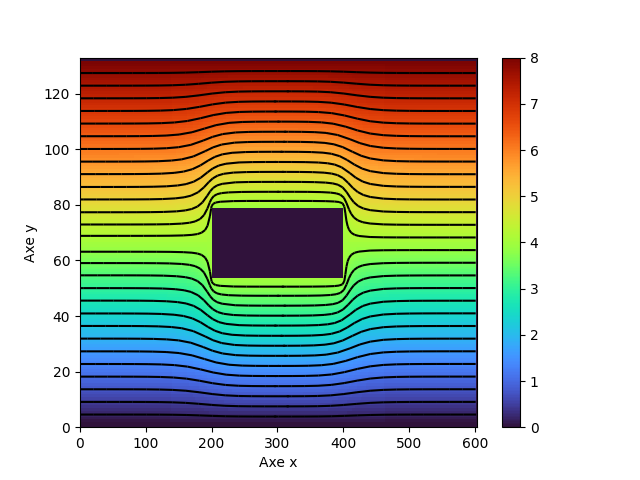
\includegraphics[width=0.5\textwidth]{"../pictures/stream2.png"}
        \caption{  Écoulement avec l'îlot au centre  }
        \label{fig1}
    \end{figure}
\pagebreak
\section*{Question 5 :}
Selon le paradoxe d'Alembert la valeur de la traînée(dans un fluide parfait) doit être nulle , il en va de même pour la portance à cause de la symétrie du problème les vitesse sont les même de chaque coté ce qui implique selon Bernoulli que les pression au dessus et en dessous de l'îlot sont égales.Un raisonement similaire peut être mené en appliquant le théorème de Kutta-Joukowski qui dit que $F_{portance}=-\rho U_{\infty} \Gamma$ et nous savons que la circulation est nul vu la symétrie.
\\ \\ Voici donc les valeur trouvées qui sont respectivement la traînée, la portance et la circulation: $8,035794252236883.10^{-13}$N; $ 4,490008365110043.10^{-11}$N; $-1,3795631303992195.10{-12}$m²/s 
\\ Nous obtenons donc des valeurs non nulles mais extrêmement petites provenant  des approximations numériques.

 \begin{figure}[h]
        \centering
        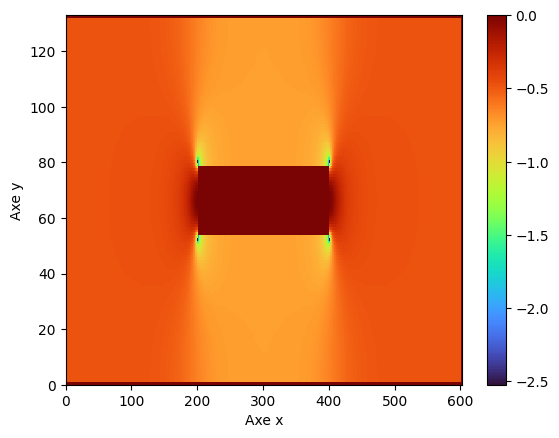
\includegraphics[width=0.5\textwidth]{"../pictures/pressure2.png"}
        \caption{Distribution de pression avec l'îlot centré   }
    \end{figure}


\section*{Question 6 :}
Le débit perpendiculaire ce réparti de la même façon qu'au cas 2, de manière égale de chaque cotés donc vu que nous conservons les même conditions limites de part et d'autre de l'ilot.
\begin{figure}[h]
        \centering
        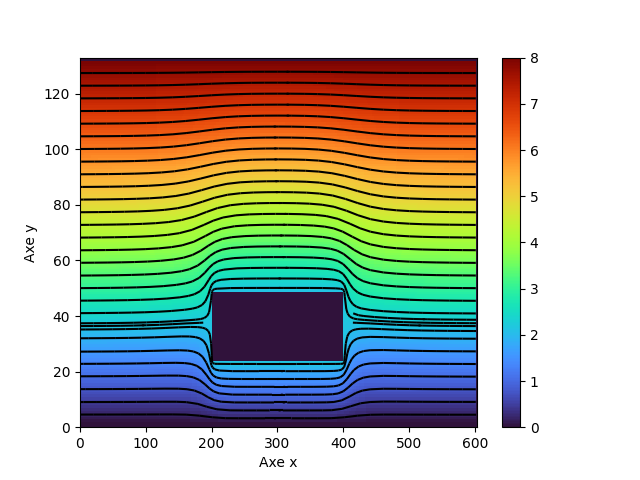
\includegraphics[width=0.6\textwidth]{"../pictures/stream3.png"}
        \caption{  Écoulement avec l'îlot décentré  }
    \end{figure}


\pagebreak
\section*{Question 7 :}

Dans ce cas la circulation n'est plus nulle ce qui implique bien une portance non nulle également . La portance est toujours nul selon le paradoxe d'Alembert puisque l'hypothèse du fluide parfait est conservé.\\ Les valeur ainsi obtenue sont pour la traînée:$ 5,728750807065808.10^{-14}$N; pour la portance:$110,4440600063123$N et pour la circulation:$-2,665568755272851$m²/s.
Encore une fois la traînée est non nulle mais très petite du aux approximations numériques.

 Par rapport au cas 2, ici l'asymétrie du problème étudié cause une circulation et une différence de vitesse de chaque coté de l'îlot du au fait que nous conservons les même conditions limites. Cela engendre alors une portance.

\begin{figure}[h]
        \centering
        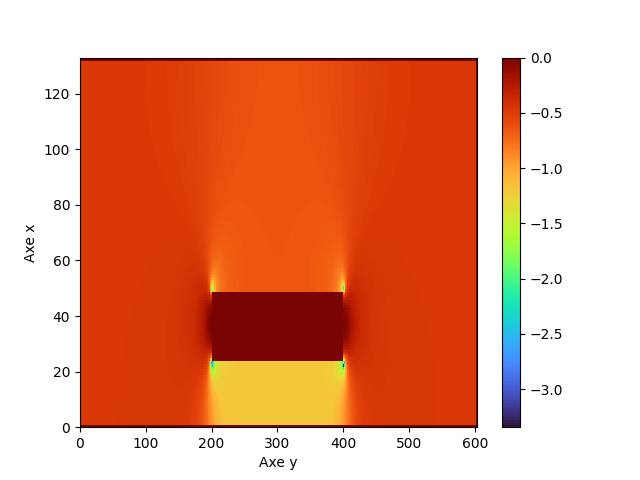
\includegraphics[width=0.5\textwidth]{"../pictures/pressure3.png"}
        \caption{Distribution de pression avec l'îlot décentré   }
    \end{figure}



\section*{Question 8 :}

La condition de Kuta consiste à vérifier l'équation suivante $\Gamma=4\pi a U_{\infty}\sin\alpha=0$, nous obtenons donc $\Gamma=0$ car l'angle d'attaque $\alpha$ est nul. On va donc itérer sur le débit de sorte à vérifier cette équation qui est l'écoulement réel, de plus à cause de l'imperméabilité de l'îlot, la valeur de la condition limite est constante sur le pourtour de l'îlot. Pour obtenir la valeur nous permettant d avoir une circulation nulle , nous avons utilisé la méthode de la bissection. On obtient une approximation numérique de la circulation de (4,216791963940203e-07 $m^2/s$) pour un débit de (1,8978822708129879 $m^2/s$).




 \begin{figure}[!h]
\begin{center}
     \begin{subfigure}[b]{0.45\textwidth}
     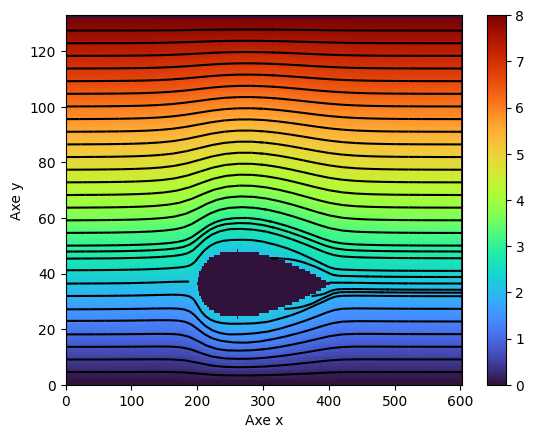
\includegraphics[width=1\textwidth]{"../pictures/stream4.png"}
     \caption{ Écoulement avec un débit=$8m^2/s$}
     \end{subfigure}
     \hfill
     \begin{subfigure}[b]{0.45\textwidth}
     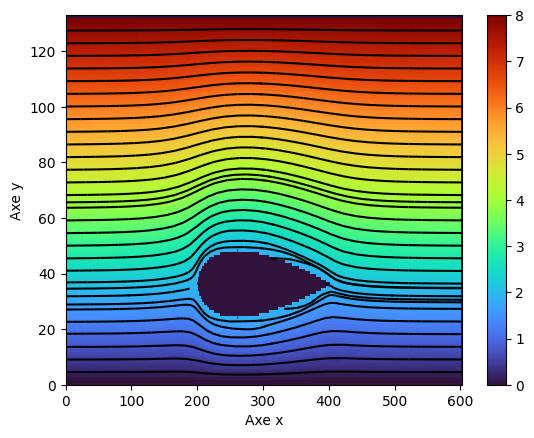
\includegraphics[width=1\textwidth]{"../pictures/stream5.png"}
     \caption{ Écoulement $\Gamma=0$, débit=$1,897 m^2/s$}
     \end{subfigure}
      \caption{ Îlot réaliste et décentré }

\end{center}
 \end{figure}


\end{document}